\documentclass[a4paper,12pt]{extarticle}
\usepackage{geometry}
\usepackage[T1]{fontenc}
\usepackage[utf8]{inputenc}
\usepackage[english,russian]{babel}
\usepackage{amsmath}
\usepackage{amsthm}
\usepackage{amssymb}
\usepackage{fancyhdr}
\usepackage{setspace}
\usepackage{graphicx}
\usepackage{colortbl}
\usepackage{tikz}
\usepackage{pgf}
\usepackage{subcaption}
\usepackage{listings}
\usepackage{indentfirst}
\usepackage[
backend=biber,
style=numeric,
maxbibnames=99
]{biblatex}
\addbibresource{refs.bib}
\usepackage[colorlinks,citecolor=blue,linkcolor=blue,bookmarks=false,hypertexnames=true, urlcolor=blue]{hyperref} 
\usepackage{indentfirst}
\usepackage{mathtools}
\usepackage{booktabs}
\usepackage[flushleft]{threeparttable}
\usepackage{tablefootnote}

\usepackage{chngcntr} % нумерация графиков и таблиц по секциям
\counterwithin{table}{section}
\counterwithin{figure}{section}

\graphicspath{{graphics/}}%путь к рисункам

\makeatletter
% \renewcommand{\@biblabel}[1]{#1.} % Заменяем библиографию с квадратных скобок на точку:
\makeatother

\geometry{left=2.5cm}% левое поле
\geometry{right=1.0cm}% правое поле
\geometry{top=2.0cm}% верхнее поле
\geometry{bottom=2.0cm}% нижнее поле
\setlength{\parindent}{1.25cm}
\renewcommand{\baselinestretch}{1.5} % междустрочный интервал


\newcommand{\bibref}[3]{\hyperlink{#1}{#2 (#3)}} % biblabel, authors, year
\addto\captionsrussian{\def\refname{Список литературы (или источников)}} 

\renewcommand{\theenumi}{\arabic{enumi}}% Меняем везде перечисления на цифра.цифра
\renewcommand{\labelenumi}{\arabic{enumi}.}% Меняем везде перечисления на цифра.цифра
\renewcommand{\theenumii}{.\arabic{enumii}}% Меняем везде перечисления на цифра.цифра
\renewcommand{\labelenumii}{\arabic{enumi}.\arabic{enumii}.}% Меняем везде перечисления на цифра.цифра
\renewcommand{\theenumiii}{.\arabic{enumiii}}% Меняем везде перечисления на цифра.цифра
\renewcommand{\labelenumiii}{\arabic{enumi}.\arabic{enumii}.\arabic{enumiii}.}% Меняем везде перечисления на цифра.цифра

\NewDocumentCommand{\codeword}{v}{
\texttt{\textcolor{blue}{#1}}
}

\NewDocumentCommand{\mono}{v}{
\texttt{\textcolor{black}{#1}}
}

\begin{document}
\begin{titlepage}
    \newpage
    
    {\setstretch{1.0}
    \begin{center}
    ПРАВИТЕЛЬСТВО РОССИЙСКОЙ ФЕДЕРАЦИИ\\
    ФГАОУ ВО НАЦИОНАЛЬНЫЙ ИССЛЕДОВАТЕЛЬСКИЙ УНИВЕРСИТЕТ\\
    «ВЫСШАЯ ШКОЛА ЭКОНОМИКИ»
    \\
    \bigskip
    Факультет компьютерных наук\\
    Образовательная программа «Машинное обучение и высоконагруженные системы»
    \end{center}
    }
    
    \vspace{2em}
    УДК 004.42
    \vspace{5em}
    
    \begin{center}
    %Выберите какой у вас проект
    %{\bf Отчет об исследовательском проекте на тему:}\\
    {\bf Отчет о программном проекте на тему:}\\
    {\bf Разработка сервиса для классификации изображений овощей}
    \end{center}
    
    \vspace{2em}
    
    {\bf Выполнил: \vspace{2mm}}
    
    {\setstretch{1.0}
    \begin{tabular}{l@{\hskip 1.5cm}c@{\hskip 1.5cm}c}
    студент & & \\
    Павлов Сергей Владимирович & \rule{3.5cm}{0.15mm}  &  \rule{3.5cm}{0.15mm} \vspace{-2mm} \\
     & \tiny{(подпись)}  & \tiny{(дата)} \\
    \end{tabular}}
    
    \vspace{1em}
    {\bf Принял руководитель проекта: \vspace{2mm}}
    
    {\setstretch{1.0}
    \begin{tabular}{l@{\hskip 1.5cm}l}
    Кантонистова Елена Олеговна\\
    Доцент\\
    Факультета компьютерных наук НИУ ВШЭ \vspace{10mm}\\
    \rule{4cm}{0.15mm}  &  \rule{4cm}{0.15mm} \vspace{-2mm}\\
    {\hskip 1.5cm}\tiny{(подпись)} & {\hskip 1.5cm}\tiny{(дата)} \\
    \end{tabular}}
    
    \vspace{\fill}
    
    \begin{center}
    Москва 2023
    \end{center}
    
    \end{titlepage}% это титульный лист - выберите подходящий вам из имеющихся в проекте вариантов
\newpage
\setcounter{page}{2}

{
	\hypersetup{linkcolor=black}
	\tableofcontents
}

\newpage

\newpage
\section*{Аннотация}   % this is how to use russian
В данной работе обозревается процесс разработки и вывода в эксплуатацию сервиса для классификации
изображений: от подготовки сериализованного экземпляра модели для получения предсказаний до
размещения пользовательского интерфейса в виде web-страницы в открытом доступе.\par

В качестве набора данных для основы проекта используется известный Vegetable Image Dataset из
сообщества Kaggle. Выбор набора данных обусловлен его готовностью к использованию без дополнительной
обработки и наличием качественных решений по его классификации от участников сообщества.\par

Кодовая база сервиса представляет собой два отдельных приложения: сервер API и web-интерфейс,
размещенные в отдельных git репозиториях. Оба приложения являются контейнеризированными и обернуты в
Helm-чарты для установки в кластерах Kubernetes. Автоматизация развертывания новых версий выполнена
с помощью GitHub Actions.\par

Акцент в данной работе сделан на качестве следущих ключевых элементов: общей программной архитектуры,
кодовых баз приложений сервиса и автоматизации процессов CI/CD. Для полноценного ознакомления с
работой рекомендуется просмотр содержимого исходного кода приложений.

\addcontentsline{toc}{section}{Аннотация}

\section*{Ключевые слова}
Классификация изображений, разработка, CI/CD, API, UI, Kubernetes, Docker, Helm, S3, PostgreSQL,
Python, PyTorch, ONNX, TypeScript, Litestar, Dramatiq, RabbitMQ, Vue, Vuetify, git, GitHub
\pagebreak

\section{Введение}

\subsection{Постановка задачи}

В рамках данной работы планируется разработать и вывести в поддерживаемую эксплуатацию сервис для
классификации изображений на базе открытого набора данных с фотографиями овощей~\cite{dataset}. План
работы состоит из следующих подзадач:

\begin{enumerate}
	\item Решить задачу классификации овощей по виду овоща (огурец, помидор и т.д.):
	\begin{enumerate}
		\item Поскольку данная задача уже хорошо отработана коллегами из сообщества Kaggle,
		воспользоваться примерами лучших архитектур для получения хорошего качества предсказаний.
		\item Имплементировать выбранную архитектуры модели на стеке, используемом в
		данной работе (Python~\cite{python}, PyTorch~\cite{pytorch}), обучить модель, оценить качество.
		\item Подготовить сериализованный объект с моделью для использования в сессиях инференса в
		в рантайме сервиса.
	\end{enumerate}
	\item Найти или разработать алгоритм, позволяющий определить доминантный «цвет» изображения
	(красный, зеленый и т.д.) и разметить при помощи него исходный набор данных. Также включить в
	процесс инференса разметку новых изображений с использованием этого алгоритма.
	\item Разработать сервер API, позволяющий:
	\begin{enumerate}
		\item Отправлять запрос с комбинацией параметров «количество + вид + цвет» и получать вывод
		изображений овощей, соответствующих предоставленной комбинации параметров. Предусмотреть
		адекватную визуализацию отсутствия подходящих изображений в базе.
		\item Загружать пользовательское изображение овоща и получать вывод его разметки по виду
		(полученной через сессию инференса) и цвету (вычисленной через имплементацию алгоритма).
	\end{enumerate}
	\item Разработать web-интерфейс сервиса для взаимодействия с сервером API через браузер.
	\item Настроить автоматизацию процессов CI/CD для сервера API и web-интерфейса.
	\item Выполнить развертывание разработанной связки API + UI на демонстрационном стенде с
	публичным сетевым адресом и провести живую презентацию работы сервиса.
\end{enumerate}

\subsection{Ожидаемые результаты}

В качестве результата задачи классификации ожидается модель на базе PyTorch, позволяющая
предсказывать вид овоща с качеством по accuracy score не менее 0.97 на данных для валидации. Модель
должна быть сериализована в формате, подходящем для запуска сессии инференса для загруженных
пользователями изображений.\par

В качестве результата разработки сервиса ожидается приложение со следующей архитектурой:

\begin{figure}[ht]
	\centering
	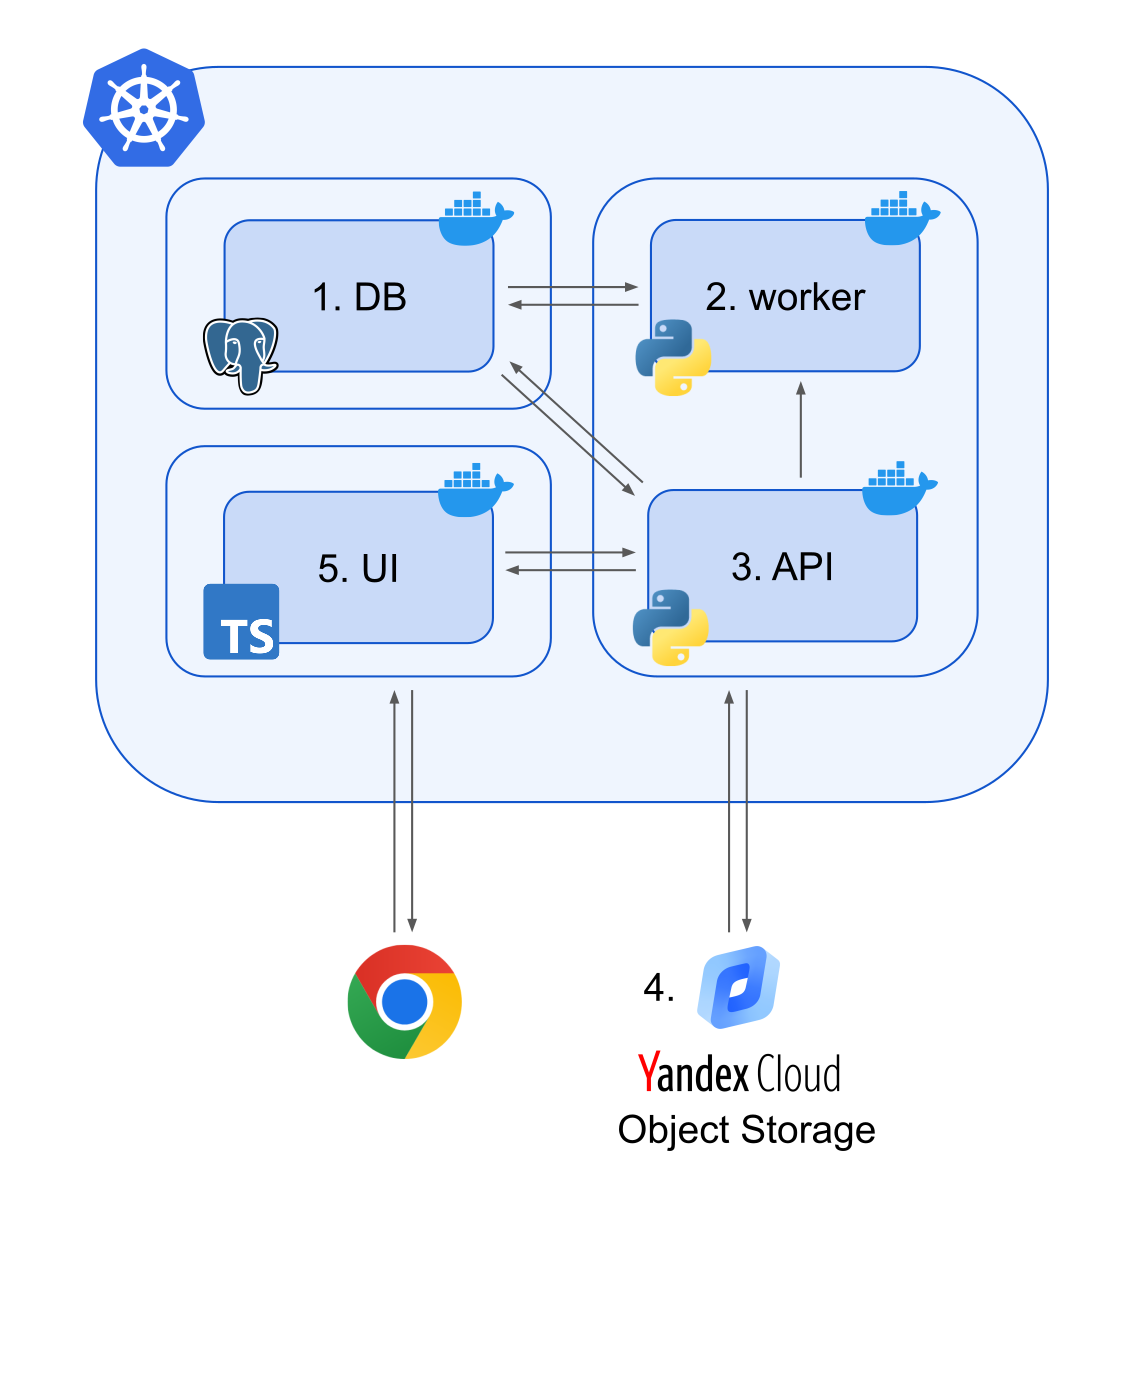
\includegraphics[width=0.8\textwidth,trim={0 2cm 0 0}]{expected_arch.png}
	\caption{Начальный план архитектуры для разрабатываемого сервиса.}
	\label{fig:expected_arch}
\end{figure}

\begin{enumerate}
	\item На рисунке~\ref{fig:expected_arch}: «1. DB». Реляционная база данных
	(например, PostgreSQL~\cite{postgresql}) для хранения метаинформации об изображениях
	(путь к файлу и разметка изображения по виду и цвету) и справочника вида овощей.
	\item На рисунке~\ref{fig:expected_arch}: «2. worker». Вспомогательный рантайм Python для выполнения
	задач в фоновом режиме на базе библиотеки Celery~\cite{celery} или аналогичного инструмента. В частности, для
	разметки загруженного пользователем изображения без задержки ответа на POST запрос.
	\item На рисунке~\ref{fig:expected_arch}: «3. API». Сервер API на базе одного из современных
	асинхронных web-фреймворков на Python, обеспечивающий основной функционал взаимодействия с
	сервисом и вызывающий исполнение фоновых задач worker-ом.
	\item На рисунке~\ref{fig:expected_arch}: «4. Object Storage». Внешнее облачное файловое хранилище
	для исходного набора фотографий и загруженных пользователями изображений. Сервис хранилища должен
	предоставлять удобный API для загрузки / чтения файлов. Также должна быть возможность генерировать
	временные ссылки для скачивания файлов, чтобы скачивание могло происходить в рантайме клиентского
	приложения. Под эти критерии подходит, например, совместимое с интерфейсом S3 хранилище от
	Yandex Cloud~\cite{storage}.
	\item На рисунке~\ref{fig:expected_arch}: «5. UI». Веб-сервер упакованных статических файлов для
	отрисовки пользовательского интерфейса в браузере. Выполнить кодовую базу UI планируется на
	TypeScript~\cite{typescript} с использованием одного из современных SPA-фреймворков.
	\item Сборка образов приложений при помощи GitHub Actions~\cite{actions} с последующим хранением артефактов в
	GitHub Container Registry (ghcr.io)~\cite{ghcr}.
	\item Автоматическое развертывания новых релизов приложений в кластере Kubernetes на личной
	машине автора через установку Helm-чартов~\cite{helm} с помощью GitHub Actions. 
	\item Доступ к сервису по протоколу HTTPS через поддомен на личном домене автора.

\end{enumerate}
	
\newpage
\section[Краткий обзор существующих решений задачи классификации]{\texorpdfstring{Краткий обзор существующих решений\\ задачи классификации}{Краткий обзор существующих решений задачи классификации}}

\subsection{Пример 1. InceptionV3 transfer learning}

Решение~\cite{example_1} с использованием архитектуры Inception V3~\cite{inceptionV3}, обученной
на открытом наборе данных ImageNet~\cite{imagenet}. В качестве предобработки исходного набора
изображений автор применил следующие преобразования:

\begin{itemize}
	\item повышение насыщенности цвета
	\item повышение контрастности
	\item повышение резкости
\end{itemize}

\begin{figure}[ht]
	\centering
	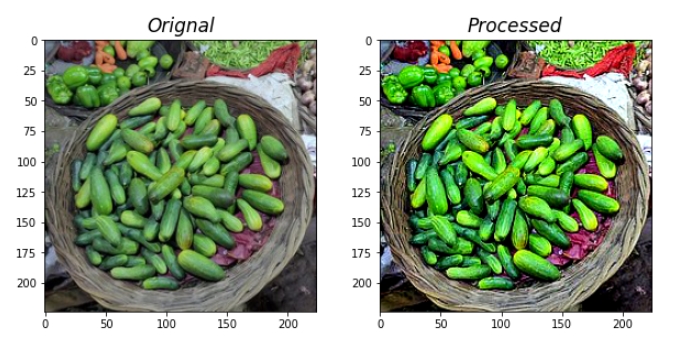
\includegraphics[width=0.8\textwidth]{example_1.png}
	\caption{Результат преобразований.}
	\label{fig:example_1}
\end{figure}

Поверх выходного слоя InceptionV3 были добавлены следующие слои:

\begin{itemize}
    \item слой 2D average pooling
    \item полносвязный слой с функцией активации ReLU
    \item слой Dropout с коэффициентом 0.2
    \item выходной полносвязный слой для классификации с Softmax
\end{itemize}

Обучение производилось в 5 эпох. В качестве функции потерь была использована категориальная
кросс-энтропия. В качестве оптимизационного алгоритма - Adam.
Полученная модель на наборе данных для валидации показала средний accuracy score в размере 0.992.
Худшее значение среди всех классов - 0.97. Лучшее значение среди всех классов - 1.00.

\newpage
\subsection{Пример 2. EfficientNet-b0 transfer learning}

Решение~\cite{example_2} с использованием модели EfficientNet-b0~\cite{efficientnet}, предобученной на ImageNet. В качестве случайных
аугментаций для исходного набора данных были использованы следующие преобразования:

\begin{itemize}
    \item горизонтальное отражение изображения
    \item изменение высоты изображения с коэффициентом 0.2
    \item изменение ширины изображения с коэффициентом 0.2
    \item поворот изображения с коэффициентом 0.2\\ и заполнением пустоты ближайшим пикселем
    \item приближение / отдаление изображения с коэффициентом 0.2
\end{itemize}

Поверх выходного слоя EfficientNet-b0 были добавлены следующие слои:

\begin{itemize}
    \item слой 2D average pooling
    \item выходной полносвязный слой для классификации с Softmax
\end{itemize}

В качестве функции потерь была использована категориальная кросс-энтропия. В качестве
оптимизационного алгоритма - Adam. Обучение производилось в 2 этапа по 5 эпох. Сначала были
использованы 20\% от исходного набора данных для обучения. После этого шага модель на наборе данных
для валидации показала средний accuracy score в размере 0.992.\par

На втором этапе веса из предыдущего обучения использовались в качестве начальных весов модели, а
набор данных для обучения был уже полным (100\% от исходного набора данных для обучения).
Архитектура самой модели относительно предыдущего этапа осталась без изменений. Результатом второго
этапа обучения стал средний accuracy score в размере 0.998 на наборе данных для валидации.

\newpage
\subsection{Пример 3. CNN}

Решение~\cite{example_3} с использованием стандартного подхода - построения пользовательской архитектуры сверточной
нейронной сети.\par

Преобразования исходного набора данных и случайные аугментации не использовались. Выбранная
архитектура слоев нейронной сети выглядела следующим образом:

\begin{table}[ht]
	\caption{Архитектура сверточной нейронной сети.}
	\label{table:example_3_arch}
	\footnotesize
	\centering
	\begin{tabular}{ |l|l|r| }
		\hline
		Тип слоя & Размерность выхода & Количество параметров \\ [0.5ex]
		\hline\hline
		Conv2D & (None, 150, 150, 32) & 896 \\
		\hline
		MaxPooling2D & (None, 75, 75, 32) & 0 \\
		\hline
		Conv2D & (None, 75, 75, 64) & 18496 \\
		\hline
		MaxPooling2D & (None, 37, 37, 64) & 0 \\
		\hline
		Flatten & (None, 87616) & 0 \\
		\hline
		Dense / Linear & (None, 128) & 11214976 \\
		\hline
		Dropout & (None, 128) & 0 \\
		\hline
		Dense / Linear & (None, 128) & 16512 \\
		\hline
		Dense / Linear & (None, 15) & 1935 \\
		\hline
	\end{tabular}
\end{table}

Обучение производилось в 100 эпох c условием остановки при отсутствии улучшения качества модели на
протяжении 5 эпох. В качестве функции потерь была использована категориальная кросс-энтропия.
В качестве оптимизационного алгоритма - Adam.\par

Обучение длилось 15 эпох. Полученная модель на наборе данных для тестирования показала средний
accuracy score в размере 0.955.

\newpage
\section{Разведочный анализ данных}

\subsection{Примеры классов}

\begin{figure}[ht]
	\centering
	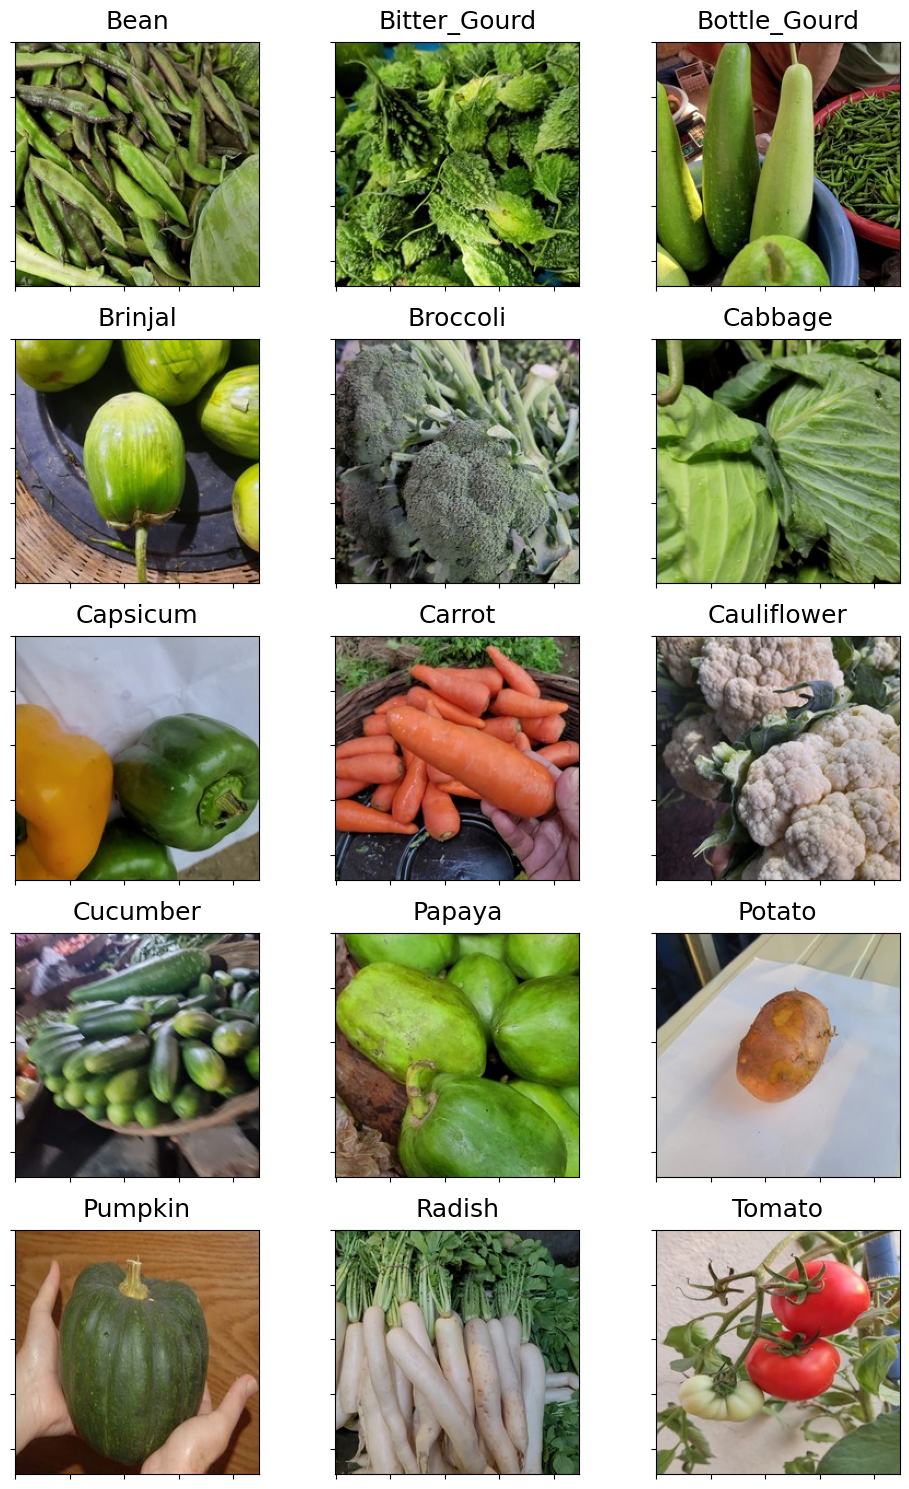
\includegraphics[width=0.65\textwidth]{EDA.png}
	\caption{Примеры изображений каждого класса из набора данных для обучения.}
	\label{fig:EDA}
\end{figure}

\newpage
\subsection{Обзор данных}

Исходный набор данных состоит из изображений 21000 изображений 15 видов овощей. Классы
сбалансированы ровно, то есть на каждый вид овоща приходится всего 1400 изображений. Исходный набор
данных изначально разделен на группы для обучения, тестирования и валидации (train, test, validation)
в отношении 70\% / 15\% / 15\%. Это 15000 / 3000 / 3000 изображений соответственно (1000 / 200 / 200
на каждый класс).\par

Ручной просмотр изображений не позволил выявить откровенные выбросы, требующие исключения из
обучения. Но точно имеют место угловые кейсы, когда несколько разных видов овощей попадаются вместе
на одной фотографии, что может привести к ошибкам в классификации.

\begin{figure}[ht]
	\centering
	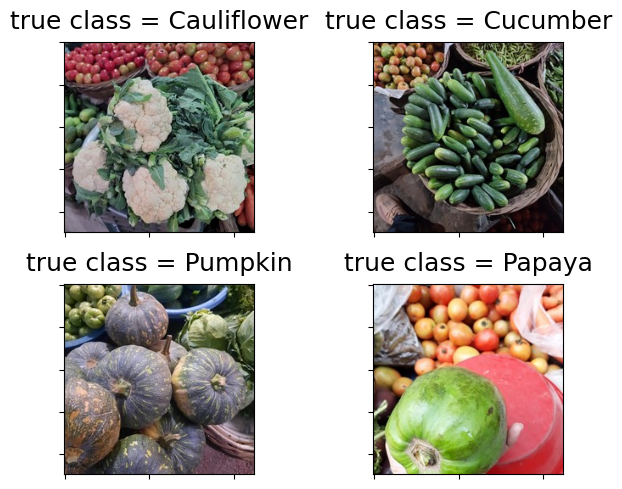
\includegraphics[width=0.8\textwidth]{EDA_outliers.png}
	\caption{Примеры cложных для классификации изображений.}
	\label{fig:EDA_outliers}
\end{figure}

\newpage
\section{Описание baseline модели}

\subsection{Архитектура модели}

В качестве основания baseline модели использовалась модель c архитектурой Inception V3, предобученная
на наборе данных ImageNet. В качестве весов использовался объект \codeword{DEFAULT} из пространства имен 
\codeword{torchvision.models.Inception_V3_Weights}. Перечисленные сущности скачивались из онлайн хаба
pytorch/vision версии 0.10.0.\par

Последний слой модели (классификатор) был заменен на полносвязный слой с размерностью выхода,
соответствующей количеству классов в используемом в данной работе наборе данных – 15.\par

Для всех изображений из набора данных было применено преобразование увеличения размера картинки до
299 на 299 пикселей, поскольку именно такую размерность модель Inception V3 ожидает на вход.\par

В качестве функции потерь была использована категориальная кросс-энтропия. В качестве
оптимизационного алгоритма - Adam. Также использовался планировщик StepLR с понижением коэффициента
скорости обучения на 0.1 каждые 5 эпох. Размер батча был равен 64.

Обучение модели производилось в бесплатном рантайме Kaggle Notebook с использованием GPU.

\subsection{Результаты обучения модели}

\begin{table}[ht]
	\caption{Результаты обучение baseline модели.}
	\label{table:baseline_by_epoch}
	\footnotesize
	\centering
	\begin{tabular}{ |r|r|r| }
		\hline
		Номер эпохи & Accuracy score на тестовых данных & Accuracy score на валидационных данных \\ [0.5ex]
		\hline\hline
		1 & 89.13\% & 98.60\% \\
		\hline
		2 & 97.38\% & 99.07\% \\
		\hline
		3 & 98.29\% & 99.30\% \\
		\hline
		4 & 98.61\% & 99.50\% \\
		\hline
		5 & 98.94\% & 99.60\% \\
		\hline
	\end{tabular}
\end{table}

\newpage
\section{Описание плана экспериментов с моделью}

\subsection{Оптимизация преобразований исходного набора данных}

В рамках baseline модели использовалось только одно преобразование – увеличение размера изображений
с $224^2$ до $299^2$. Даже такой простейший подход показал отличный результат – 99.60\% accuracy
score на валидационных данных.\par

Тем не менее, в библиотеке torchvision в имеется метод \codeword{transforms} из
пространства имен \codeword{torchvision.models.Inception_V3_Weights.IMAGENET1K_V1},
возвращающий набор готовых преобразований для инференса на архитектуре Inception V3. Можно попробовать
включить в пайплайн применение этих преобразований и оценить изменения качества предсказаний.

\newpage
\section{Результаты экспериментов c моделью}

\subsection{Оптимизация преобразований исходного набора данных}

В пайплайн были добавлены рекомендованные для Inception V3 документацией библиотеки PyTorch
преобразования.\par

Список преобразований:

\begin{itemize}
	\item Увеличение размера изображения до $342^2$
	\item Central crop размера (299, 299)
	\item Масштабирование числовых значений пикселей на шкалу [0.0, 1.0]
	\item Нормализация со средним [0.485, 0.456, 0.406]\\
	и стандартным отклонением [0.229, 0.224, 0.225]
\end{itemize}

C данными преобразованиями обучение модели показало следующий результат:

\begin{table}[ht]
	\caption{Результаты обучение baseline модели c использованием преобразований.}
	\label{table:baseline_transformed_by_epoch}
	\footnotesize
	\centering
	\begin{tabular}{ |r|r|r| }
		\hline
		Номер эпохи & Accuracy score на тестовых данных & Accuracy score на валидационных данных \\ [0.5ex]
		\hline\hline
		1 & 89.57\% & 98.43\% \\
		\hline
		2 & 97.57\% & 99.17\% \\
		\hline
		3 & 98.17\% & 99.37\% \\
		\hline
		4 & 98.56\% & 99.63\% \\
		\hline
		5 & 98.71\% & 99.57\% \\
		\hline
	\end{tabular}
\end{table}

Можно резюмировать, что применение к входным данным рекомендованных для данной
архитектуры преобразований значимо не повлияло на качество модели.

Финальная архитектура модели и логика обучения ее обучения хранятся в формате Jupyter Notebook в
контроле версий проекта~\cite{model}.

\newpage
\section{Алгоритм определения доминантного цвета}

\subsection{Палитры цветов}

Доминантный цвет изображений определяется по двум разным популярным цветовым палитрам отдельно
(по каждой палитре свой доминантный цвет).

\subsubsection{RGB}

\begin{table}[ht]
	\caption{Палитра цветов RGB.}
	\label{table:RGB}
	\footnotesize
	\centering
	\begin{tabular}{ |l|r|r|r| }
		\hline
		hex & red & green & blue \\ [0.5ex]
		\hline\hline
		\mono{#FF0000} & 255 & 0 & 0 \\
		\hline
		\mono{#FF8000} & 255 & 128 & 0 \\
		\hline
		\mono{#FFFF00} & 255 & 255 & 0 \\
		\hline
		\mono{#80FF00} & 128 & 255 & 0 \\
		\hline
		\mono{#00FF00} & 0 & 255 & 0 \\
		\hline
		\mono{#00FF80} & 0 & 255 & 128 \\
		\hline
		\mono{#00FFFF} & 0 & 255 & 255 \\
		\hline
		\mono{#0080FF} & 0 & 128 & 255 \\
		\hline
		\mono{#0000FF} & 0 & 0 & 255 \\
		\hline
		\mono{#8000FF} & 128 & 0 & 255 \\
		\hline
		\mono{#FF00FF} & 255 & 0 & 255 \\
		\hline
		\mono{#FF0080} & 255 & 0 & 128 \\
		\hline
	\end{tabular}
\end{table}

\begin{figure}[ht]
	\centering
	
\includegraphics[width=0.5\textwidth]{RGB.png}
	\caption{Палитра цветов RGB.}
	\label{fig:RGB}
\end{figure}

\newpage
\subsubsection{RYB}

\begin{table}[ht]
	\caption{Палитра цветов RYB.}
	\label{table:RYB}
	\footnotesize
	\centering
	\begin{tabular}{ |l|r|r|r| }
		\hline
		hex & red & green & blue \\ [0.5ex]
		\hline\hline
		\mono{#FE2712} & 254 & 39 & 18 \\
		\hline
		\mono{#FC600A} & 252 & 96 & 10 \\
		\hline
		\mono{#FB9902} & 251 & 153 & 2 \\
		\hline
		\mono{#FCCC1A} & 252 & 204 & 26 \\
		\hline
		\mono{#FEFE33} & 254 & 254 & 51 \\
		\hline
		\mono{#B2D732} & 178 & 215 & 50 \\
		\hline
		\mono{#66B032} & 102 & 176 & 50 \\
		\hline
		\mono{#347C98} & 52 & 124 & 152 \\
		\hline
		\mono{#0247FE} & 2 & 71 & 254 \\
		\hline
		\mono{#4424D6} & 68 & 36 & 214 \\
		\hline
		\mono{#8601AF} & 134 & 1 & 175 \\
		\hline
		\mono{#C21460} & 194 & 20 & 96 \\
		\hline
	\end{tabular}
\end{table}

\begin{figure}[ht]
	\centering
	
\includegraphics[width=0.5\textwidth]{RYB.png}
	\caption{Палитра цветов RYB.}
	\label{fig:RYB}
\end{figure}

\newpage
\subsection{Описание алгоритма}

Алгоритм определения доминантного цвета основан на вычислении евклидового расстояния в трехмерном
пространстве (reg, green, blue) между пикселями изображений и точками, соответствующими цветам в
выбранной палитре.\par

Цвет, для которого его среднее расстояние является наименьшим среди всех цветов палитры, выбирается
в качестве доминантного, и его hex код записывается в базу данных.

\subsection{Имплементация алгоритма}

\begin{figure}[ht]
	\centering
	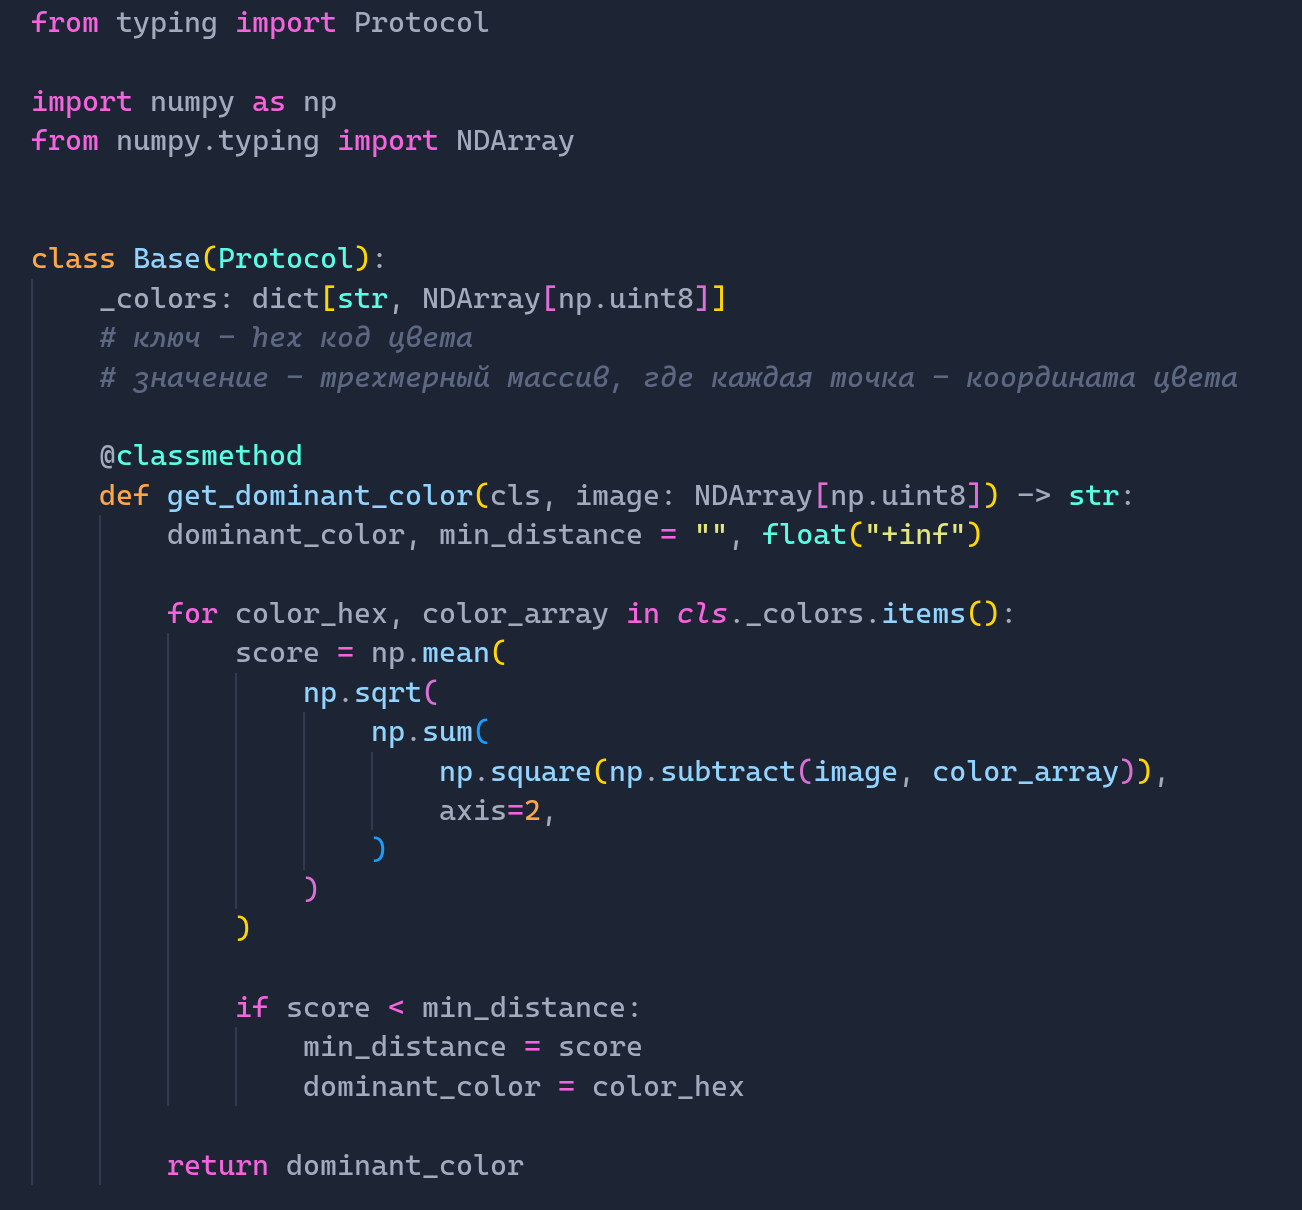
\includegraphics[width=0.8\textwidth]{color_utils.png}
	\caption{Имплементация базового utility-класса для вычисления доминантного цвета.}
	\label{fig:color_utils}
\end{figure}

Логика алгоритма вынесена в отдельную библиотеку~\cite{color_utils} для переиспользования:

\begin{itemize}
	\item в среде основного проекта для разметки исходного набора данных
	\item в среде сервера API для разметки загружаемых пользователями изображений
\end{itemize}

\newpage
\section{Описание реализованной архитектуры сервиса}

\subsection{Организация кодовой базы проекта}

В родительском репозитории~\cite{gradwork} данной работы находится среда Python для запуска разметки
исходного набора данных по доминантным цветам. Там же хранятся исходники данного текста в исходном
формате LaTeX и сопутствующие артефакты.\par

Кодовые базы приложений сервера API и web-интерфейса подключены в родительской репозиторий в качестве
подмодулей git~\cite{submodules}.

\subsection{Хранение изображений}

Исходный набор данных скачан с публичного реестра Kaggle и размещен в приватном хранилище Yandex
Cloud Object Storage. Данный тип хранилища имеет интерфейс, совместимый с AWS S3,
поэтому для доступа к изображениям из среды приложения используется Python-библиотека
boto3~\cite{boto3}.\par

В рамках сервера API реализован интерфейс~\cite{coreS3} для чтения и записи изображений, а также для
получение временной ссылки на скачивание одного изображения без авторизации.

\subsection{Сериализация экземпляра обученной модели}

После обучения модели ее объект сериализуется в формат, совместимый с ONNX Runtime~\cite{ONNX}, с
помощью метода \codeword{torch.onnx.export}. Сериализованный экземпляр модели хранится в том же
Object Storage, что используется и для хранения изображений.

\subsection{Развертывание cервиса}

Сервер API~\cite{server} и web-интерфейс~\cite{web_UI} являются отдельными приложениями и,
соответственно, их релизы устанавливаются отдельными Helm-чартами~\cite{server_chart,web_UI_chart} в
кластер Kubernetes на личной машине автора данной работы.\par

Автоматизация сборки образов и развертывания / обновления релизов выполнена на базе GitHub Actions в
репозиториях сервера API~\cite{server_CI} и web-интерфейса~\cite{web_UI_CI}. Образы приложений
хранятся в GitHub Container Registry~\cite{github_packages}.

\newpage
\subsection{Cхема архитектуры cервиса}

\begin{figure}[ht]
	\centering
	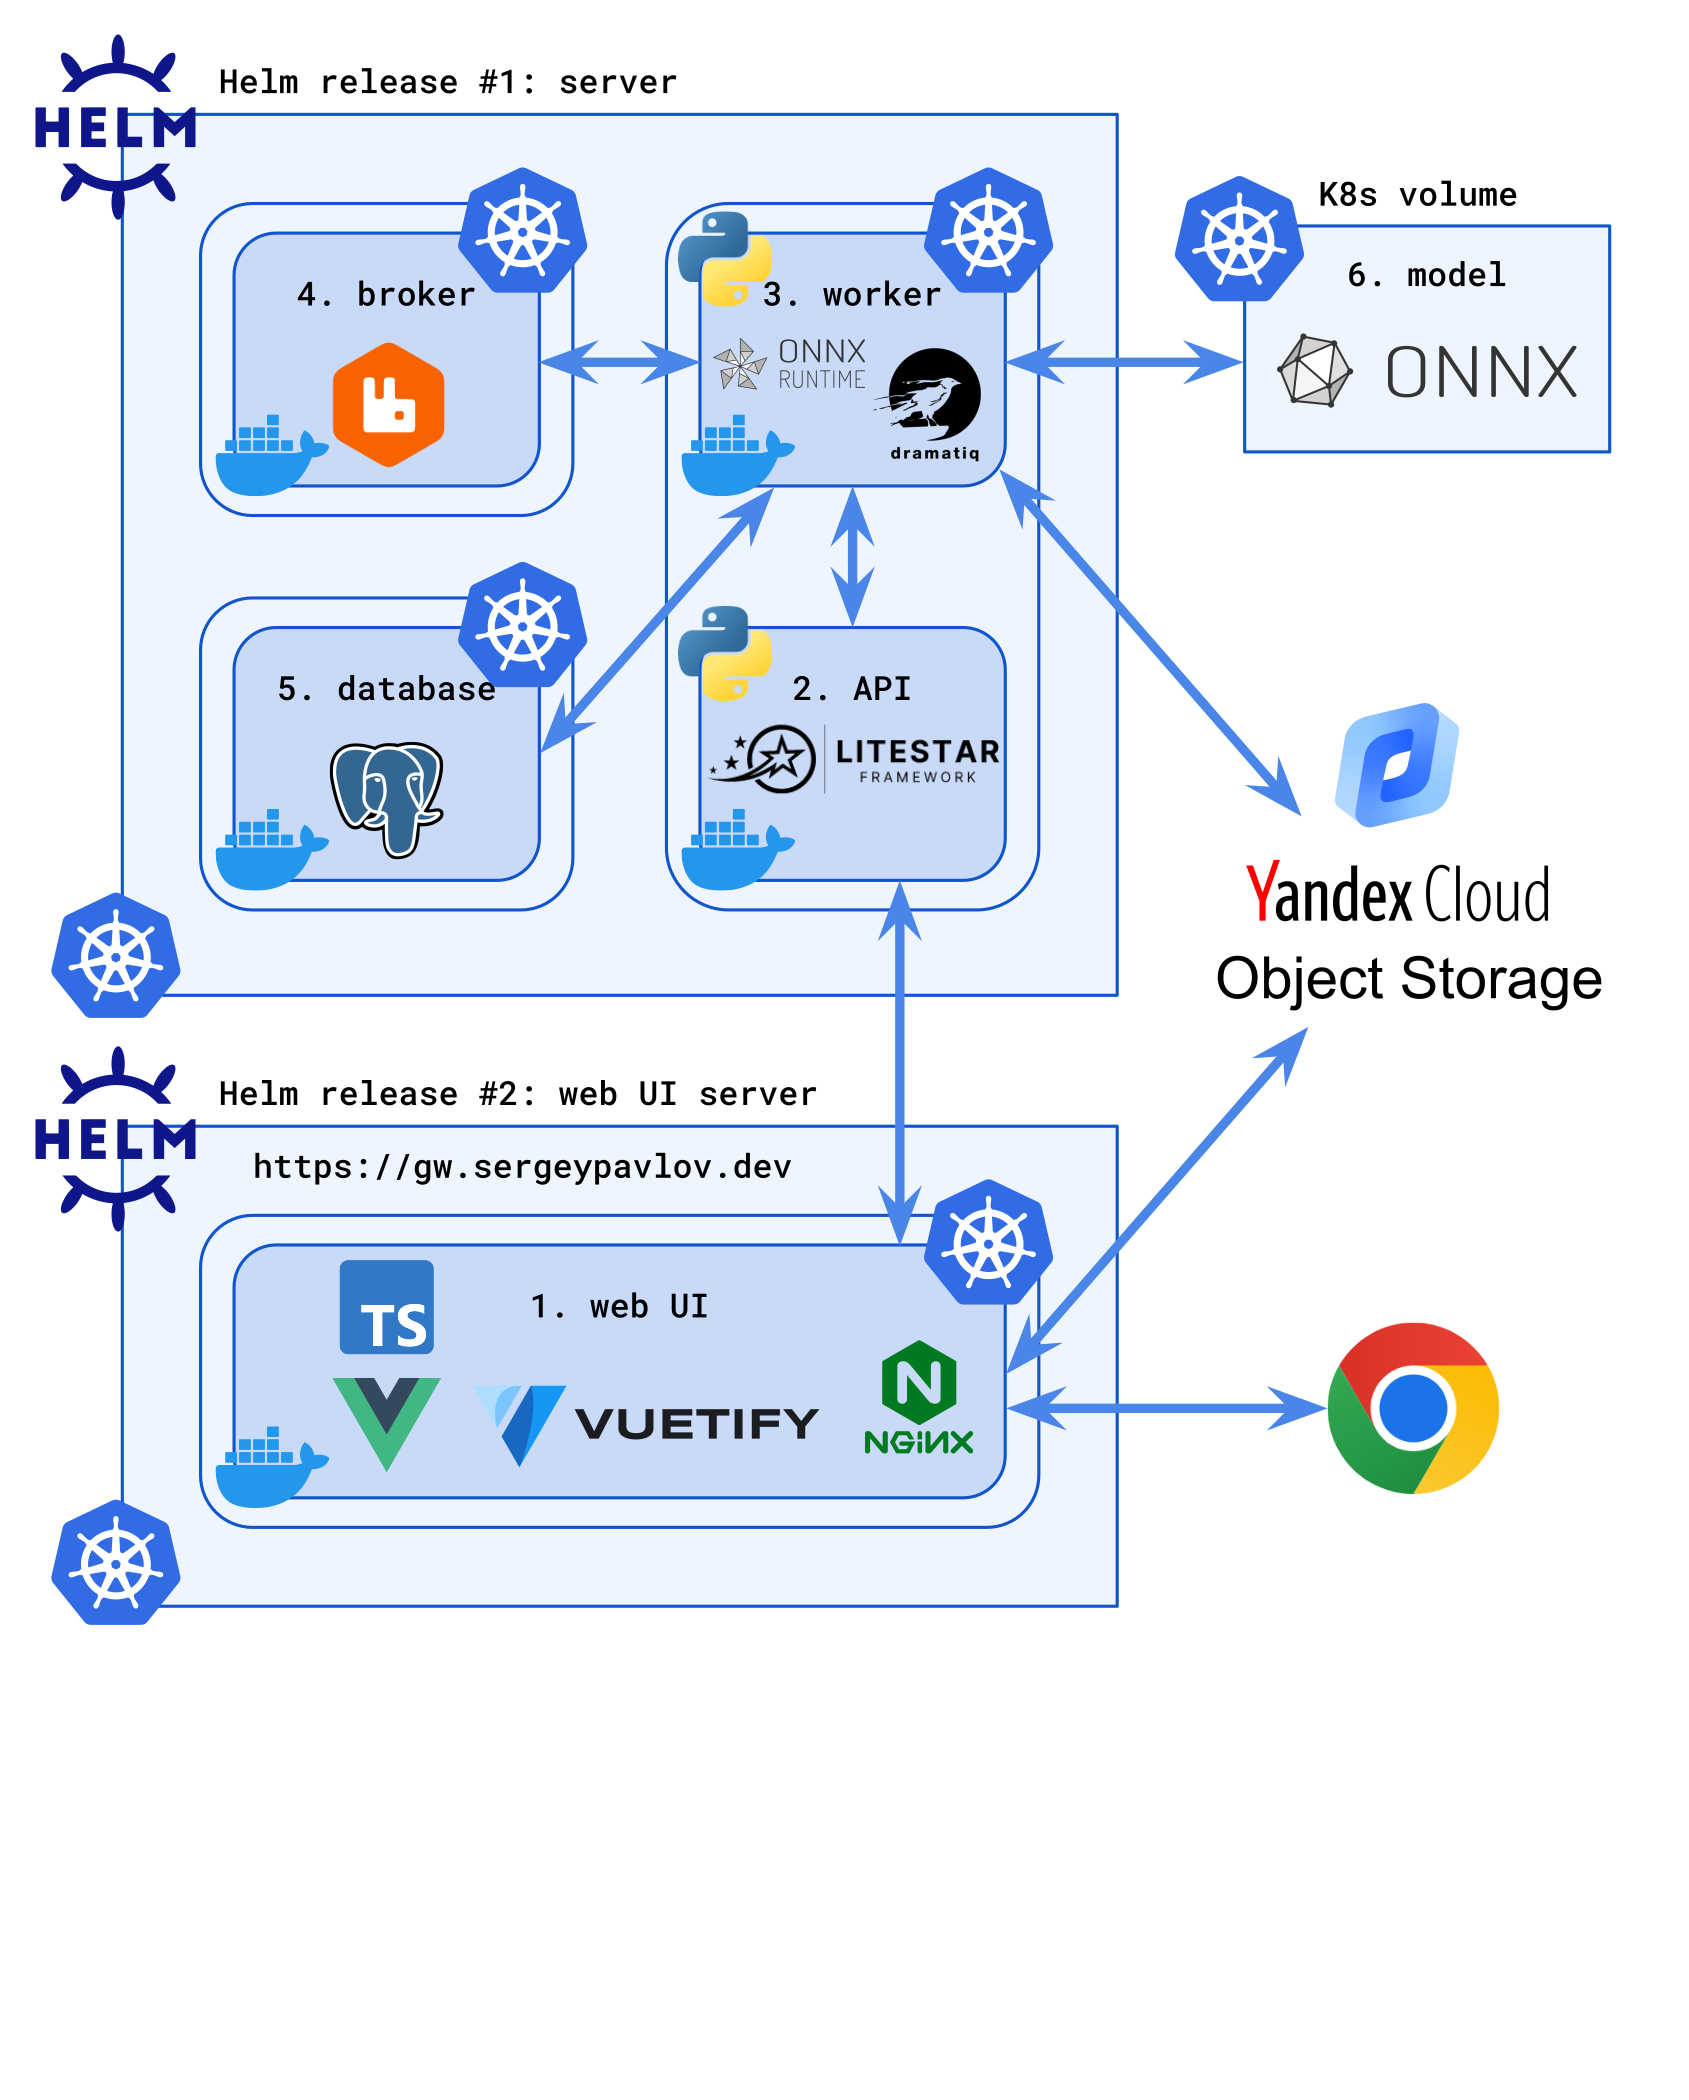
\includegraphics[width=0.95\textwidth,trim={0 3.5cm 0 0}]{final_arch.png}
	\caption{Схема финальной архитектуры сервиса.}
	\label{fig:final_arch}
\end{figure}

\subsubsection{Web UI}

На рисунке~\ref{fig:final_arch}: «1. web UI». Для пользователя точкой входа для взаимодействия с
приложением является web-интерфейс, доступный на одном из поддоменов личного домена
автора~\cite{hosted}. Запросы статических файлов браузером для рендера web-интерфейса обсуживаются
web-сервером NGINX~\cite{NGINX}.\par

Логика web-интерфейса выполнена на языке TypeScript на базе фреймворка Vue.js~\cite{vue} и с
использованием библиотеки готовых UI-компонентов Vuetify~\cite{vuetify}.\par

Выбор данного стека обусловлен исключительно желанием автора данной работы попробовать frontend
технологии, с которыми он не имел дела в контексте основной профессиональной деятельности. Иначе
имело бы смысл воспользоваться самым популярным web-фреймворком для single page applications в
экосистеме JavaScript, которым на текущий момент заслуженно остается~\cite{stateofjs}
React~\cite{react}.\par

В web-интерфейсе реализовано две вкладки (рис.~\ref{fig:tabs}) для двух основных элементов
функционала:

\begin{itemize}
	\item просмотр исходного набора данных с возможностью фильтрации по:
	\begin{itemize}
		\item количеству выводимых изображений (от 1 до 9)
		\item классу овоща
		\item доминантному цвету изображения по палитре RGB или RYB
	\end{itemize} 
	\item загрузка пользовательского изображения и визулизация результата его классификации и
	разметки по цвету
\end{itemize}

\begin{figure}[ht]
	\centering
	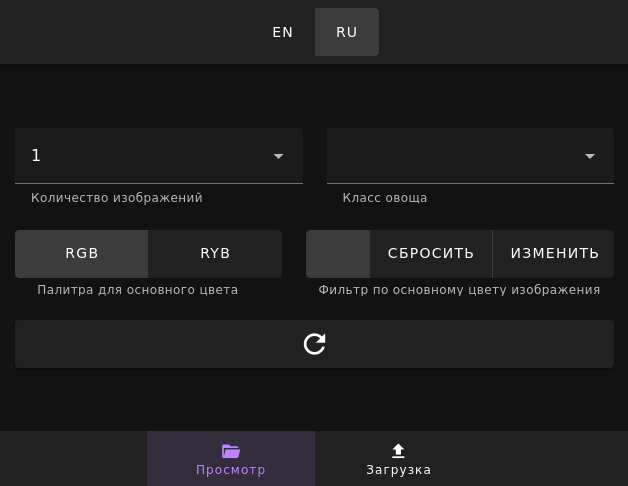
\includegraphics[width=0.45\textwidth,height=6.5cm]{tab_browse.png}
	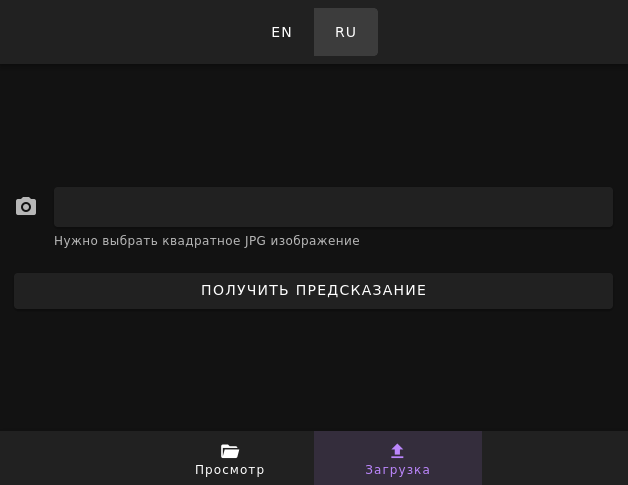
\includegraphics[width=0.45\textwidth,height=6.5cm]{tab_upload.png}
	\caption{Вкладки web-интерфейса.}
	\label{fig:tabs}
\end{figure}

\subsubsection{Сервер API}

На рисунке~\ref{fig:final_arch}: «2. API». Действия, выполняемые пользователем в web-интерфейсе,
отправляют запросы из браузера пользователя к серверу API приложения. Логика сервера API выполнена
на языке Python с использованием web-фреймворка Litestar~\cite{litestar}.\par

Рантайм сервера API обеспечивается процессами WSGI HTTP сервера Gunicorn~\cite{gunicorn} с
использованием класса воркеров UvicornWorker. Это необходимо для совместимости с интерфейсом ASGI,
который является расширением интерфейса WSGI для web-приложений, использующих асинхронный функционал
Python.

Litestar (ранее называвшийся Starlite) по перечню функционала очень похож на популярный в данный
момент FastAPI~\cite{fastapi}, и изначально оба фреймворка были основаны на легковесном
ASGI-совместимом фреймворке Starlette~\cite{starlette} (Litestar на данный момент уже освобожден от
этой зависимости, что является плюсом). Также в Litestar (в отличие от FastAPI) есть поддержка
class-based контроллеров, что является классическим подходом ООП к дизайну CRUD API для сущностей
объектной модели приложения.

\subsubsection{Процессы для выполнения фоновых задач}

На рисунке~\ref{fig:final_arch}: «3. worker». Контейнер с процессом для запуска фоновых задач
работает как sidecar относительно контейнера с сервером API. В рамках рантайма сервера API
предусмотрена отправка сигналов на выполнение двух типов фоновых задач:

\begin{enumerate}
	\item сохранение загруженного пользователем изображения в S3-хранилище
	\item разметка загруженного пользователем изображения по классу овоща по доминантному цвету,
	а также запись этих результатов в базу данных
\end{enumerate}

Исполнение фоновых задач осуществляется процессами, вызываемыми с помощью Python-библиотеки
Dramatiq~\cite{dramatiq}. Для инференса внутри процессов используются сессии ONNX Runtime. Сам файл
с моделью помещается в Persistent Volume~\cite{pv} в процессе инициализации основного приложения
и считывается процессом фоновой задачи для каждого запуска сессии инференса.

\subsubsection{Менеджер очередей сообщений}

На рисунке~\ref{fig:final_arch}: «4. broker». Менеджер очередей сообщений RabbitMQ~\cite{rabbitmq},
обрабатывающий сигналы на запуск фоновых задач, поступающие из рантайма сервера API.

\subsubsection{База данных}

На рисунке~\ref{fig:final_arch}: «5. database». База данных PostgreSQL. Хранит информацию об
изображениях из исходного набора данных и о загруженных пользователем в таблице IMAGE. Есть
справочная таблица CATEGORY со списком всех классов овощей, на одну строку которой ссылается каждая
запись из таблицы IMAGE через \codeword{FOREIGN KEY}. Также таблица IMAGE содержит hex коды
доминантных цветов изображения по палитрам RGB и RYB.\par

Данные базы хранятся в локальном Persistent Volume сервера. При удалении релиза сервера API данные
сохраняются и могут быть использованы при повторной установке. Lifecycle данного volume управляется
Helm-чартом PostgreSQL, входящим как компонент в чарт сервера API.

\newpage 
\printbibliography[heading=bibintoc] 
	
\end{document}
